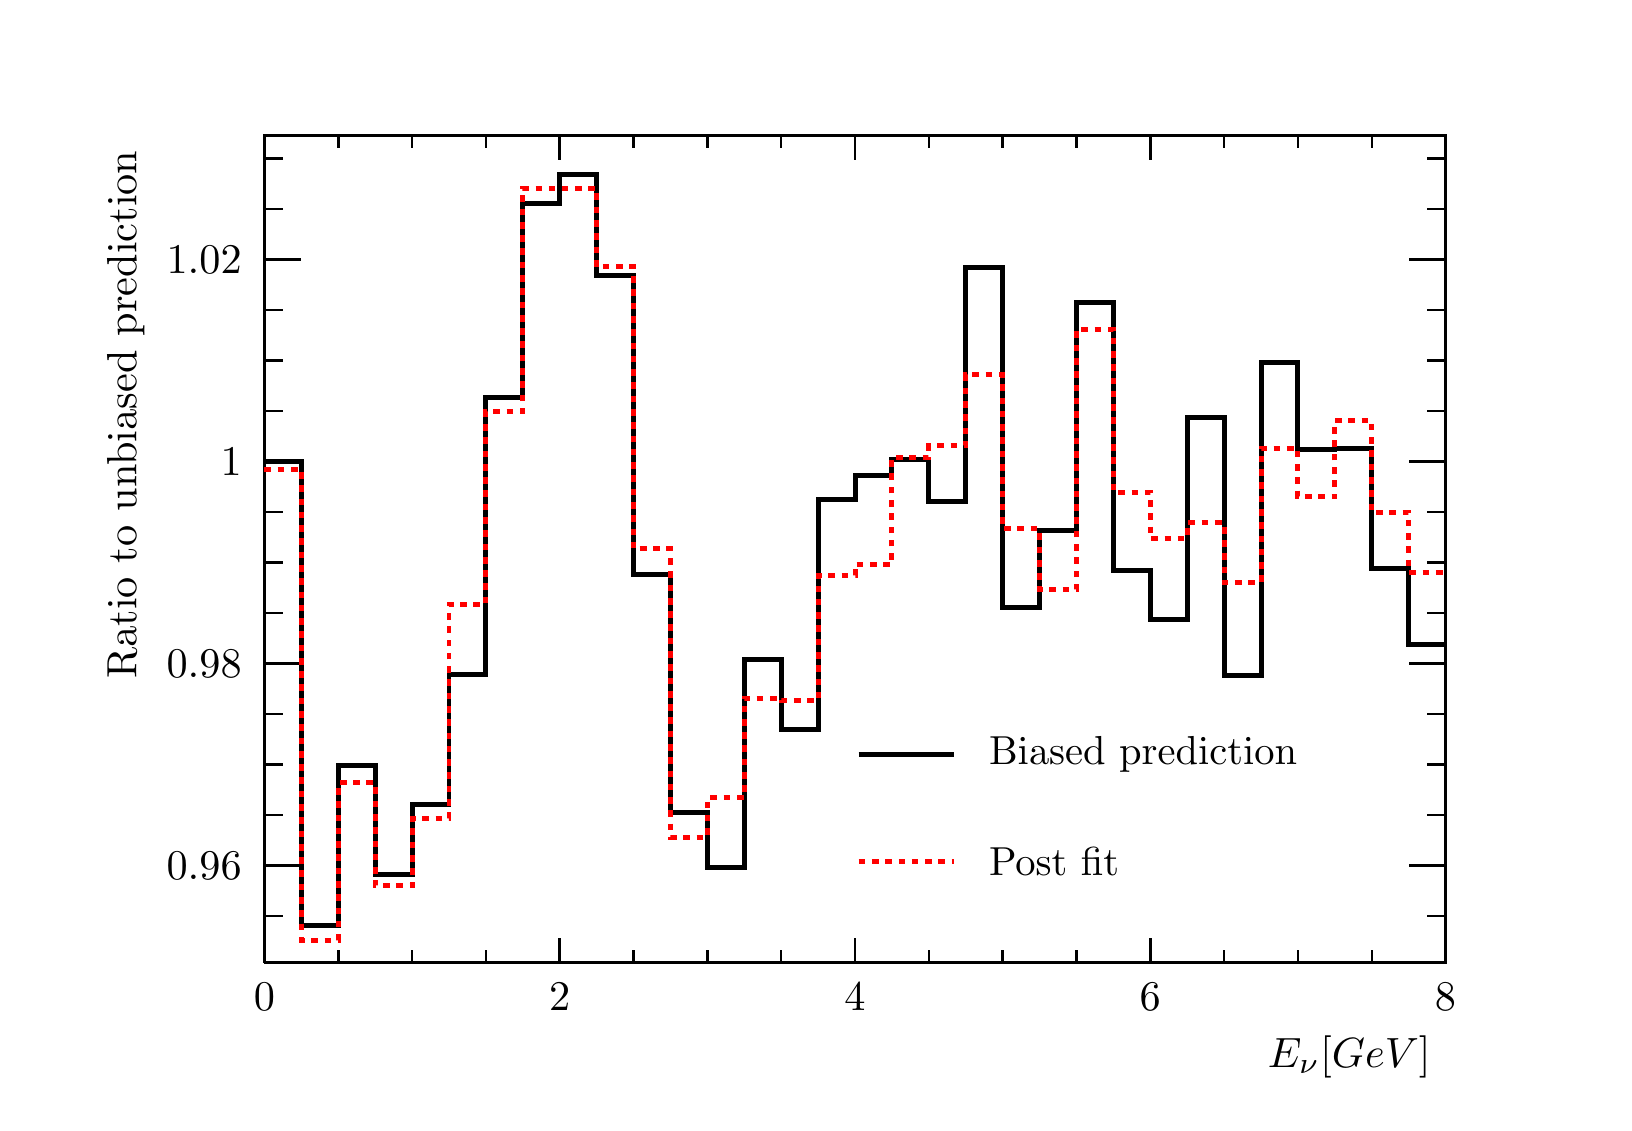
\begin{tikzpicture}
\pgfdeclareplotmark{cross} {
\pgfpathmoveto{\pgfpoint{-0.3\pgfplotmarksize}{\pgfplotmarksize}}
\pgfpathlineto{\pgfpoint{+0.3\pgfplotmarksize}{\pgfplotmarksize}}
\pgfpathlineto{\pgfpoint{+0.3\pgfplotmarksize}{0.3\pgfplotmarksize}}
\pgfpathlineto{\pgfpoint{+1\pgfplotmarksize}{0.3\pgfplotmarksize}}
\pgfpathlineto{\pgfpoint{+1\pgfplotmarksize}{-0.3\pgfplotmarksize}}
\pgfpathlineto{\pgfpoint{+0.3\pgfplotmarksize}{-0.3\pgfplotmarksize}}
\pgfpathlineto{\pgfpoint{+0.3\pgfplotmarksize}{-1.\pgfplotmarksize}}
\pgfpathlineto{\pgfpoint{-0.3\pgfplotmarksize}{-1.\pgfplotmarksize}}
\pgfpathlineto{\pgfpoint{-0.3\pgfplotmarksize}{-0.3\pgfplotmarksize}}
\pgfpathlineto{\pgfpoint{-1.\pgfplotmarksize}{-0.3\pgfplotmarksize}}
\pgfpathlineto{\pgfpoint{-1.\pgfplotmarksize}{0.3\pgfplotmarksize}}
\pgfpathlineto{\pgfpoint{-0.3\pgfplotmarksize}{0.3\pgfplotmarksize}}
\pgfpathclose
\pgfusepathqstroke
}
\pgfdeclareplotmark{cross*} {
\pgfpathmoveto{\pgfpoint{-0.3\pgfplotmarksize}{\pgfplotmarksize}}
\pgfpathlineto{\pgfpoint{+0.3\pgfplotmarksize}{\pgfplotmarksize}}
\pgfpathlineto{\pgfpoint{+0.3\pgfplotmarksize}{0.3\pgfplotmarksize}}
\pgfpathlineto{\pgfpoint{+1\pgfplotmarksize}{0.3\pgfplotmarksize}}
\pgfpathlineto{\pgfpoint{+1\pgfplotmarksize}{-0.3\pgfplotmarksize}}
\pgfpathlineto{\pgfpoint{+0.3\pgfplotmarksize}{-0.3\pgfplotmarksize}}
\pgfpathlineto{\pgfpoint{+0.3\pgfplotmarksize}{-1.\pgfplotmarksize}}
\pgfpathlineto{\pgfpoint{-0.3\pgfplotmarksize}{-1.\pgfplotmarksize}}
\pgfpathlineto{\pgfpoint{-0.3\pgfplotmarksize}{-0.3\pgfplotmarksize}}
\pgfpathlineto{\pgfpoint{-1.\pgfplotmarksize}{-0.3\pgfplotmarksize}}
\pgfpathlineto{\pgfpoint{-1.\pgfplotmarksize}{0.3\pgfplotmarksize}}
\pgfpathlineto{\pgfpoint{-0.3\pgfplotmarksize}{0.3\pgfplotmarksize}}
\pgfpathclose
\pgfusepathqfillstroke
}
\pgfdeclareplotmark{newstar} {
\pgfpathmoveto{\pgfqpoint{0pt}{\pgfplotmarksize}}
\pgfpathlineto{\pgfqpointpolar{44}{0.5\pgfplotmarksize}}
\pgfpathlineto{\pgfqpointpolar{18}{\pgfplotmarksize}}
\pgfpathlineto{\pgfqpointpolar{-20}{0.5\pgfplotmarksize}}
\pgfpathlineto{\pgfqpointpolar{-54}{\pgfplotmarksize}}
\pgfpathlineto{\pgfqpointpolar{-90}{0.5\pgfplotmarksize}}
\pgfpathlineto{\pgfqpointpolar{234}{\pgfplotmarksize}}
\pgfpathlineto{\pgfqpointpolar{198}{0.5\pgfplotmarksize}}
\pgfpathlineto{\pgfqpointpolar{162}{\pgfplotmarksize}}
\pgfpathlineto{\pgfqpointpolar{134}{0.5\pgfplotmarksize}}
\pgfpathclose
\pgfusepathqstroke
}
\pgfdeclareplotmark{newstar*} {
\pgfpathmoveto{\pgfqpoint{0pt}{\pgfplotmarksize}}
\pgfpathlineto{\pgfqpointpolar{44}{0.5\pgfplotmarksize}}
\pgfpathlineto{\pgfqpointpolar{18}{\pgfplotmarksize}}
\pgfpathlineto{\pgfqpointpolar{-20}{0.5\pgfplotmarksize}}
\pgfpathlineto{\pgfqpointpolar{-54}{\pgfplotmarksize}}
\pgfpathlineto{\pgfqpointpolar{-90}{0.5\pgfplotmarksize}}
\pgfpathlineto{\pgfqpointpolar{234}{\pgfplotmarksize}}
\pgfpathlineto{\pgfqpointpolar{198}{0.5\pgfplotmarksize}}
\pgfpathlineto{\pgfqpointpolar{162}{\pgfplotmarksize}}
\pgfpathlineto{\pgfqpointpolar{134}{0.5\pgfplotmarksize}}
\pgfpathclose
\pgfusepathqfillstroke
}
\definecolor{c}{rgb}{1,1,1};
\draw [color=c, fill=c] (0,0) rectangle (20,13.639);
\draw [color=c, fill=c] (3,1.77307) rectangle (18,12.2751);
\definecolor{c}{rgb}{0,0,0};
\draw [c,line width=0.9] (3,1.77307) -- (3,12.2751) -- (18,12.2751) -- (18,1.77307) -- (3,1.77307);
\definecolor{c}{rgb}{1,1,1};
\draw [color=c, fill=c] (3,1.77307) rectangle (18,12.2751);
\definecolor{c}{rgb}{0,0,0};
\draw [c,line width=0.9] (3,1.77307) -- (3,12.2751) -- (18,12.2751) -- (18,1.77307) -- (3,1.77307);
\draw [c,line width=1.8] (3,8.13473) -- (3.46875,8.13473) -- (3.46875,2.24935) -- (3.9375,2.24935) -- (3.9375,4.27843) -- (4.40625,4.27843) -- (4.40625,2.89272) -- (4.875,2.89272) -- (4.875,3.78438) -- (5.34375,3.78438) -- (5.34375,5.42819) --
 (5.8125,5.42819) -- (5.8125,8.94926) -- (6.28125,8.94926) -- (6.28125,11.4108) -- (6.75,11.4108) -- (6.75,11.775) -- (7.21875,11.775) -- (7.21875,10.4999) -- (7.6875,10.4999) -- (7.6875,6.7042) -- (8.15625,6.7042) -- (8.15625,3.6728) --
 (8.625,3.6728) -- (8.625,2.97665) -- (9.09375,2.97665) -- (9.09375,5.62651) -- (9.5625,5.62651) -- (9.5625,4.73508) -- (10.0312,4.73508) -- (10.0312,7.64853) -- (10.5,7.64853) -- (10.5,7.95419) -- (10.9688,7.95419) -- (10.9688,8.1559) --
 (11.4375,8.1559) -- (11.4375,7.63293) -- (11.9062,7.63293) -- (11.9062,10.6008) -- (12.375,10.6008) -- (12.375,6.28378) -- (12.8438,6.28378) -- (12.8438,7.26247) -- (13.3125,7.26247) -- (13.3125,10.1584) -- (13.7812,10.1584) -- (13.7812,6.75198) --
 (14.25,6.75198) -- (14.25,6.12528) -- (14.7188,6.12528) -- (14.7188,8.69801) -- (15.1875,8.69801) -- (15.1875,5.41503) -- (15.6562,5.41503) -- (15.6562,9.38806) -- (16.125,9.38806) -- (16.125,8.29131) -- (16.5938,8.29131) -- (16.5938,8.30536) --
 (17.0625,8.30536) -- (17.0625,6.77958) -- (17.5312,6.77958) -- (17.5312,5.81722) -- (18,5.81722);
\draw [c,line width=0.9] (3,1.77307) -- (18,1.77307);
\draw [c,line width=0.9] (3,2.07994) -- (3,1.77307);
\draw [c,line width=0.9] (3.9375,1.9265) -- (3.9375,1.77307);
\draw [c,line width=0.9] (4.875,1.9265) -- (4.875,1.77307);
\draw [c,line width=0.9] (5.8125,1.9265) -- (5.8125,1.77307);
\draw [c,line width=0.9] (6.75,2.07994) -- (6.75,1.77307);
\draw [c,line width=0.9] (7.6875,1.9265) -- (7.6875,1.77307);
\draw [c,line width=0.9] (8.625,1.9265) -- (8.625,1.77307);
\draw [c,line width=0.9] (9.5625,1.9265) -- (9.5625,1.77307);
\draw [c,line width=0.9] (10.5,2.07994) -- (10.5,1.77307);
\draw [c,line width=0.9] (11.4375,1.9265) -- (11.4375,1.77307);
\draw [c,line width=0.9] (12.375,1.9265) -- (12.375,1.77307);
\draw [c,line width=0.9] (13.3125,1.9265) -- (13.3125,1.77307);
\draw [c,line width=0.9] (14.25,2.07994) -- (14.25,1.77307);
\draw [c,line width=0.9] (15.1875,1.9265) -- (15.1875,1.77307);
\draw [c,line width=0.9] (16.125,1.9265) -- (16.125,1.77307);
\draw [c,line width=0.9] (17.0625,1.9265) -- (17.0625,1.77307);
\draw [c,line width=0.9] (18,2.07994) -- (18,1.77307);
\draw [anchor=base] (3,1.15931) node[scale=1.52731, color=c, rotate=0]{0};
\draw [anchor=base] (6.75,1.15931) node[scale=1.52731, color=c, rotate=0]{2};
\draw [anchor=base] (10.5,1.15931) node[scale=1.52731, color=c, rotate=0]{4};
\draw [anchor=base] (14.25,1.15931) node[scale=1.52731, color=c, rotate=0]{6};
\draw [anchor=base] (18,1.15931) node[scale=1.52731, color=c, rotate=0]{8};
\draw [anchor= east] (18,0.572837) node[scale=1.52731, color=c, rotate=0]{$E_{\nu} [GeV]$};
\draw [c,line width=0.9] (3,12.2751) -- (18,12.2751);
\draw [c,line width=0.9] (3,11.9682) -- (3,12.2751);
\draw [c,line width=0.9] (3.9375,12.1216) -- (3.9375,12.2751);
\draw [c,line width=0.9] (4.875,12.1216) -- (4.875,12.2751);
\draw [c,line width=0.9] (5.8125,12.1216) -- (5.8125,12.2751);
\draw [c,line width=0.9] (6.75,11.9682) -- (6.75,12.2751);
\draw [c,line width=0.9] (7.6875,12.1216) -- (7.6875,12.2751);
\draw [c,line width=0.9] (8.625,12.1216) -- (8.625,12.2751);
\draw [c,line width=0.9] (9.5625,12.1216) -- (9.5625,12.2751);
\draw [c,line width=0.9] (10.5,11.9682) -- (10.5,12.2751);
\draw [c,line width=0.9] (11.4375,12.1216) -- (11.4375,12.2751);
\draw [c,line width=0.9] (12.375,12.1216) -- (12.375,12.2751);
\draw [c,line width=0.9] (13.3125,12.1216) -- (13.3125,12.2751);
\draw [c,line width=0.9] (14.25,11.9682) -- (14.25,12.2751);
\draw [c,line width=0.9] (15.1875,12.1216) -- (15.1875,12.2751);
\draw [c,line width=0.9] (16.125,12.1216) -- (16.125,12.2751);
\draw [c,line width=0.9] (17.0625,12.1216) -- (17.0625,12.2751);
\draw [c,line width=0.9] (18,11.9682) -- (18,12.2751);
\draw [c,line width=0.9] (3,1.77307) -- (3,12.2751);
\draw [c,line width=0.9] (3.462,3.00444) -- (3,3.00444);
\draw [c,line width=0.9] (3.231,3.64573) -- (3,3.64573);
\draw [c,line width=0.9] (3.231,4.28701) -- (3,4.28701);
\draw [c,line width=0.9] (3.231,4.9283) -- (3,4.9283);
\draw [c,line width=0.9] (3.462,5.56959) -- (3,5.56959);
\draw [c,line width=0.9] (3.231,6.21087) -- (3,6.21087);
\draw [c,line width=0.9] (3.231,6.85216) -- (3,6.85216);
\draw [c,line width=0.9] (3.231,7.49344) -- (3,7.49344);
\draw [c,line width=0.9] (3.462,8.13473) -- (3,8.13473);
\draw [c,line width=0.9] (3.231,8.77601) -- (3,8.77601);
\draw [c,line width=0.9] (3.231,9.4173) -- (3,9.4173);
\draw [c,line width=0.9] (3.231,10.0586) -- (3,10.0586);
\draw [c,line width=0.9] (3.462,10.6999) -- (3,10.6999);
\draw [c,line width=0.9] (3.462,3.00444) -- (3,3.00444);
\draw [c,line width=0.9] (3.231,2.36316) -- (3,2.36316);
\draw [c,line width=0.9] (3.462,10.6999) -- (3,10.6999);
\draw [c,line width=0.9] (3.231,11.3412) -- (3,11.3412);
\draw [c,line width=0.9] (3.231,11.9824) -- (3,11.9824);
\draw [anchor= east] (2.9,3.00444) node[scale=1.52731, color=c, rotate=0]{0.96};
\draw [anchor= east] (2.9,5.56959) node[scale=1.52731, color=c, rotate=0]{0.98};
\draw [anchor= east] (2.9,8.13473) node[scale=1.52731, color=c, rotate=0]{1};
\draw [anchor= east] (2.9,10.6999) node[scale=1.52731, color=c, rotate=0]{1.02};
\draw [anchor= east] (1.24,12.2751) node[scale=1.52731, color=c, rotate=90]{Ratio to unbiased prediction};
\draw [c,line width=0.9] (18,1.77307) -- (18,12.2751);
\draw [c,line width=0.9] (17.538,3.00444) -- (18,3.00444);
\draw [c,line width=0.9] (17.769,3.64573) -- (18,3.64573);
\draw [c,line width=0.9] (17.769,4.28701) -- (18,4.28701);
\draw [c,line width=0.9] (17.769,4.9283) -- (18,4.9283);
\draw [c,line width=0.9] (17.538,5.56959) -- (18,5.56959);
\draw [c,line width=0.9] (17.769,6.21087) -- (18,6.21087);
\draw [c,line width=0.9] (17.769,6.85216) -- (18,6.85216);
\draw [c,line width=0.9] (17.769,7.49344) -- (18,7.49344);
\draw [c,line width=0.9] (17.538,8.13473) -- (18,8.13473);
\draw [c,line width=0.9] (17.769,8.77601) -- (18,8.77601);
\draw [c,line width=0.9] (17.769,9.4173) -- (18,9.4173);
\draw [c,line width=0.9] (17.769,10.0586) -- (18,10.0586);
\draw [c,line width=0.9] (17.538,10.6999) -- (18,10.6999);
\draw [c,line width=0.9] (17.538,3.00444) -- (18,3.00444);
\draw [c,line width=0.9] (17.769,2.36316) -- (18,2.36316);
\draw [c,line width=0.9] (17.538,10.6999) -- (18,10.6999);
\draw [c,line width=0.9] (17.769,11.3412) -- (18,11.3412);
\draw [c,line width=0.9] (17.769,11.9824) -- (18,11.9824);
\definecolor{c}{rgb}{1,0,0};
\draw [c,dash pattern=on 2.40pt off 2.40pt ,line width=1.8] (3,8.04085) -- (3.46875,8.04085) -- (3.46875,2.05603) -- (3.9375,2.05603) -- (3.9375,4.05462) -- (4.40625,4.05462) -- (4.40625,2.74782) -- (4.875,2.74782) -- (4.875,3.59814) --
 (5.34375,3.59814) -- (5.34375,6.3235) -- (5.8125,6.3235) -- (5.8125,8.76872) -- (6.28125,8.76872) -- (6.28125,11.608) -- (6.75,11.608) -- (6.75,11.6033) -- (7.21875,11.6033) -- (7.21875,10.6068) -- (7.6875,10.6068) -- (7.6875,7.02826) --
 (8.15625,7.02826) -- (8.15625,3.36321) -- (8.625,3.36321) -- (8.625,3.86314) -- (9.09375,3.86314) -- (9.09375,5.13095) -- (9.5625,5.13095) -- (9.5625,5.09705) -- (10.0312,5.09705) -- (10.0312,6.68316) -- (10.5,6.68316) -- (10.5,6.83127) --
 (10.9688,6.83127) -- (10.9688,8.18553) -- (11.4375,8.18553) -- (11.4375,8.33635) -- (11.9062,8.33635) -- (11.9062,9.23997) -- (12.375,9.23997) -- (12.375,7.27951) -- (12.8438,7.27951) -- (12.8438,6.50539) -- (13.3125,6.50539) -- (13.3125,9.80946) --
 (13.7812,9.80946) -- (13.7812,7.74818) -- (14.25,7.74818) -- (14.25,7.1531) -- (14.7188,7.1531) -- (14.7188,7.35722) -- (15.1875,7.35722) -- (15.1875,6.59979) -- (15.6562,6.59979) -- (15.6562,8.30161) -- (16.125,8.30161) -- (16.125,7.68726) --
 (16.5938,7.68726) -- (16.5938,8.65468) -- (17.0625,8.65468) -- (17.0625,7.48932) -- (17.5312,7.48932) -- (17.5312,6.73083) -- (18,6.73083);
\definecolor{c}{rgb}{1,1,1};
\draw [color=c, fill=c] (10.2865,2.37822) rectangle (17.2206,5.10029);
\definecolor{c}{rgb}{0,0,0};
\draw [anchor= west] (12.0201,4.41977) node[scale=1.46368, color=c, rotate=0]{Biased prediction};
\draw [c,line width=1.8] (10.5466,4.41977) -- (11.76,4.41977);
\draw [anchor= west] (12.0201,3.05874) node[scale=1.46368, color=c, rotate=0]{Post fit};
\definecolor{c}{rgb}{1,0,0};
\draw [c,dash pattern=on 2.40pt off 2.40pt ,line width=1.8] (10.5466,3.05874) -- (11.76,3.05874);
\end{tikzpicture}
